
\section{Methodology}
\label{sec:methodology}

This proposed triple heterogeneous software stack follows a high performance middleware design pattern. By specifically focusing on the orchestration of distributed classical resources alongside remote, cloud based quantum backends, we can address the preestablished "Communication Wall" \cite{weder2021quantum} through the development of an asynchronous and parallel pipeline that executes the hybrid quantum-classical software. 

\subsection{Distributed System Architecture}
This stack follows a modular architecture designed to decouple the classical, high performance subroutines from the quantum circuit execution. There are three distinct layers defined within the architecture: the Orchestration layer, the Acceleration layer, and the Quantum interface layer. This system is designed specifically to handle varying timescales of GPU accelerated classical math (microseconds), MPI interode communication (milliseconds), and cloud based QPU Round-Trip Time (RTT)(seconds). This stack moves beyond the single host, synchronous execution model found in the previous examples of hybrid middleware (like XACC) \cite{mccaskey2018xacc} that were explored in this paper's Literature Review. 

\begin{figure}[htbp]
    \centering
    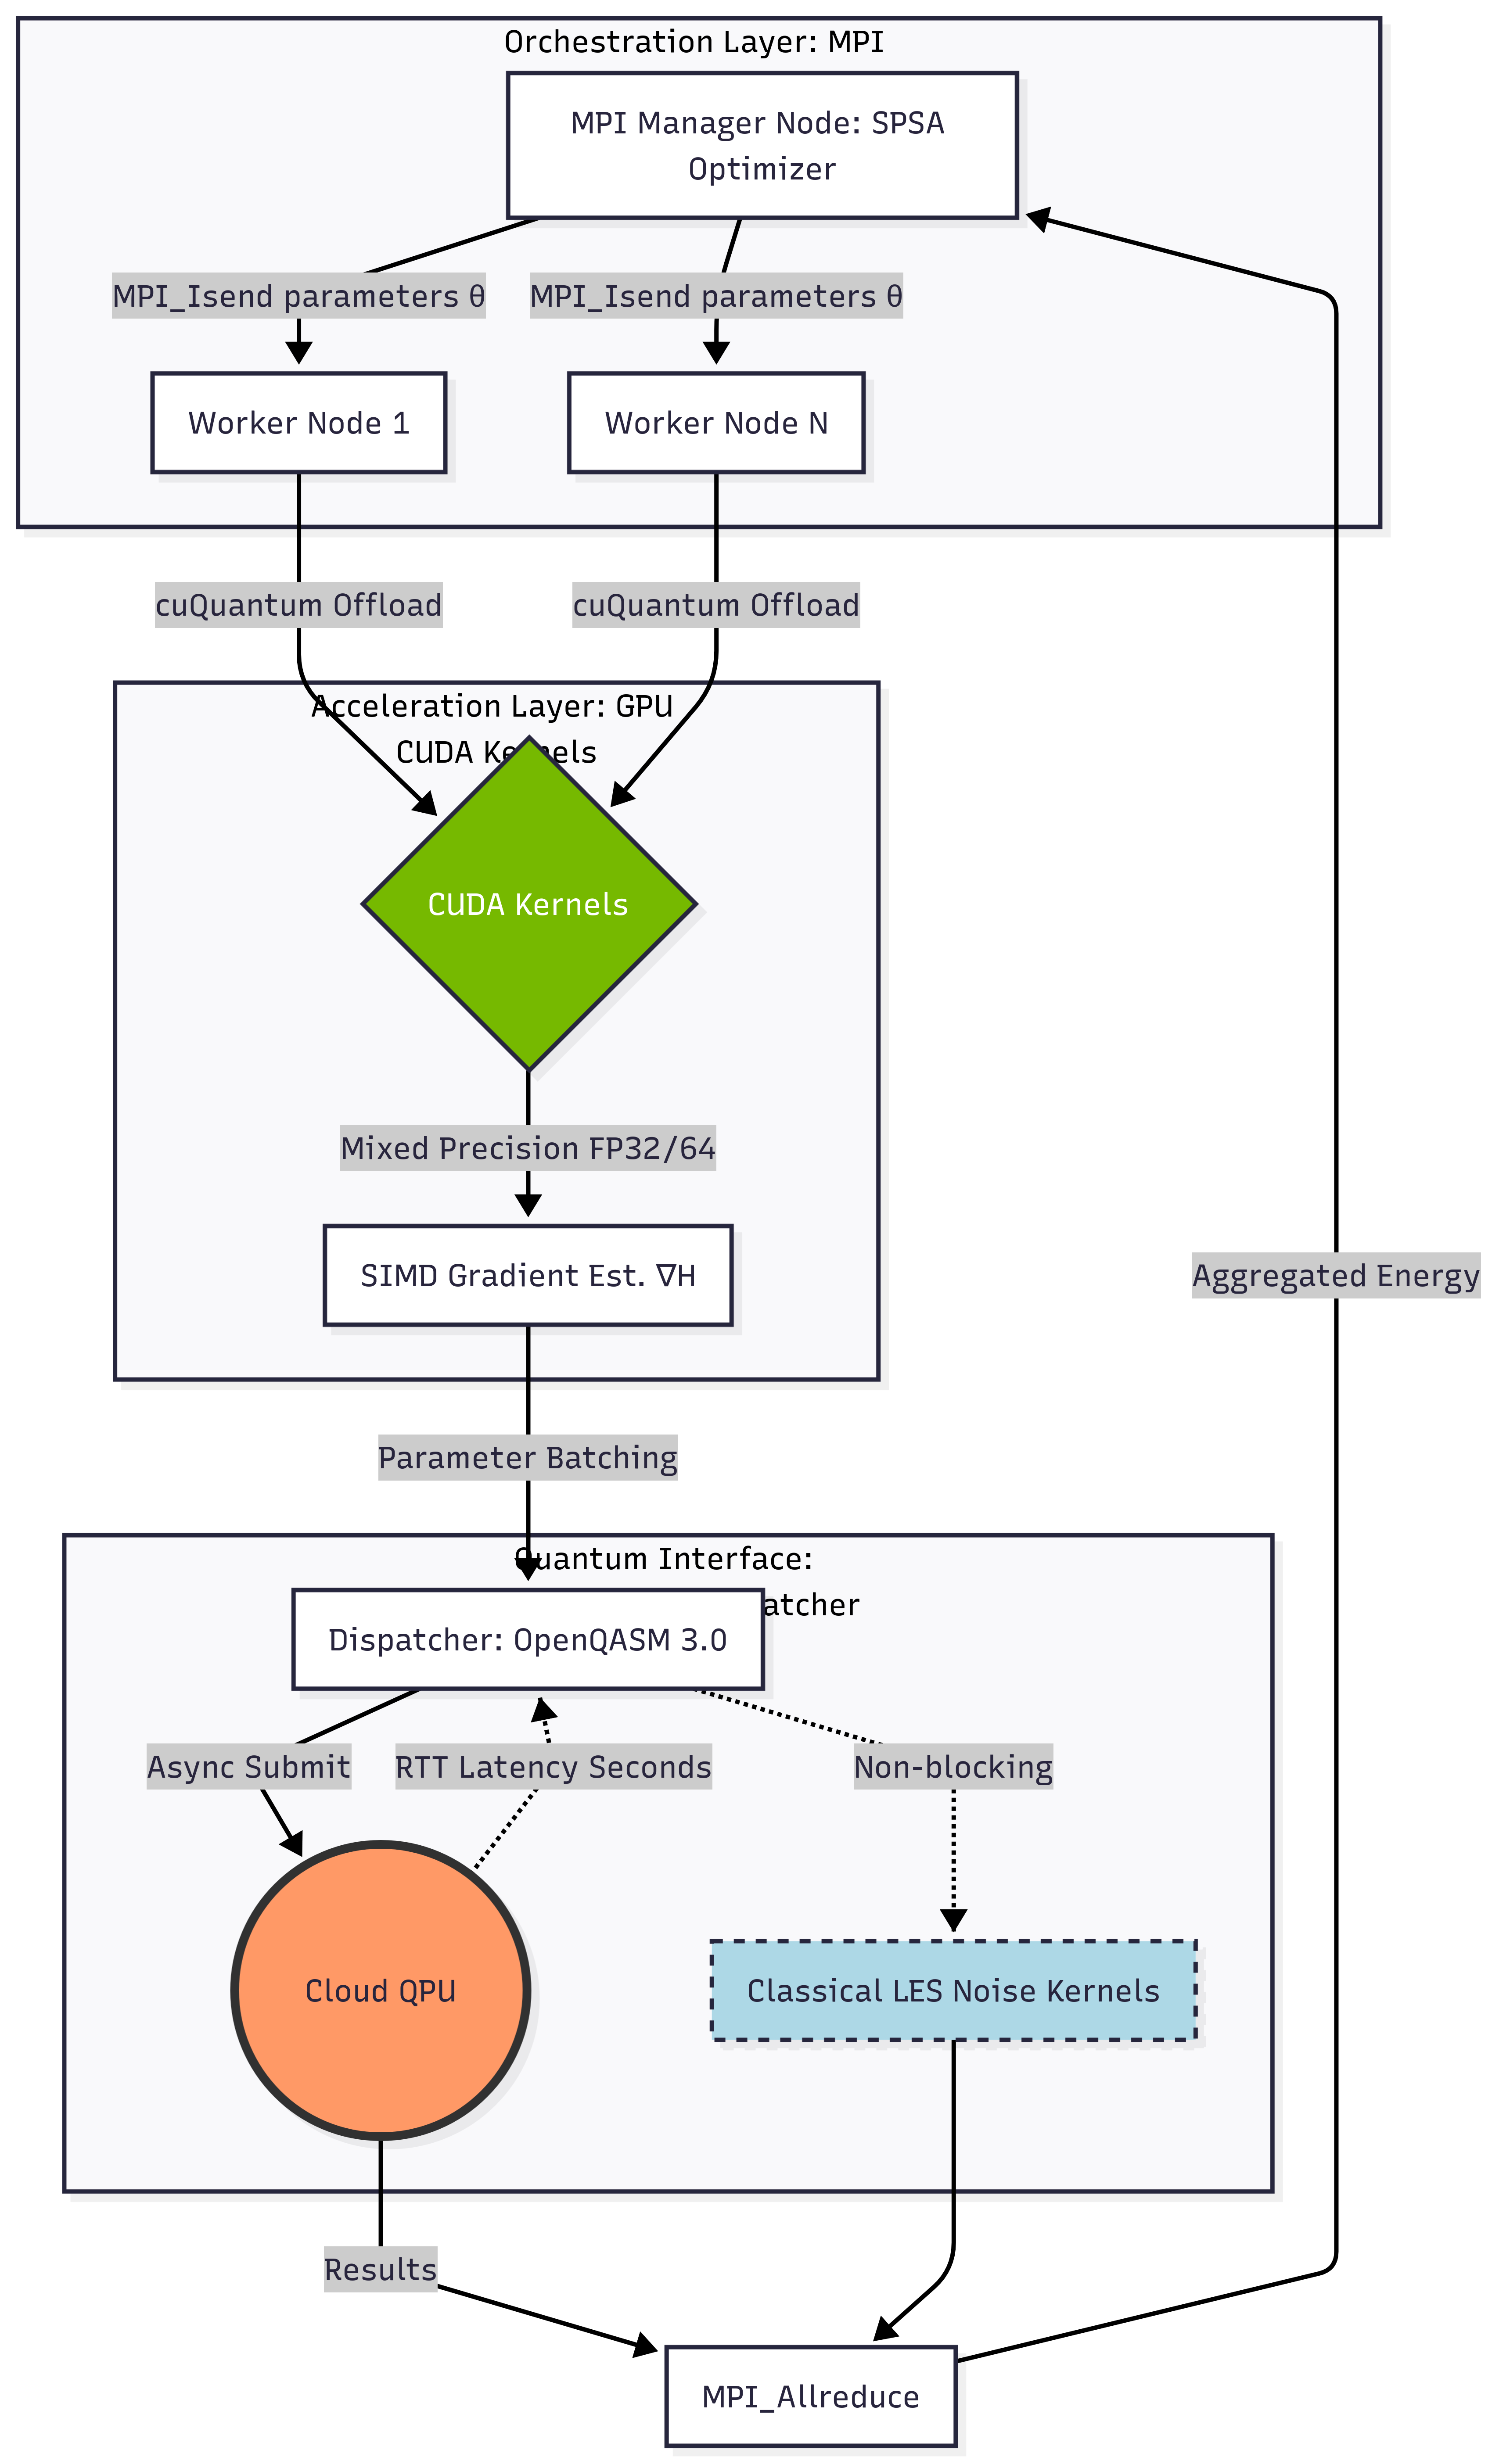
\includegraphics[width=0.8\textwidth]{graphics/system_arch_diagram.png} 
    \caption{Triple Heterogeneous System Architecture.}
    \label{fig:system_architecture}
\end{figure}


\subsubsection{Orchestration Layer: Distributed Memory and MPI Manager-Worker Topology}
This top-level layer implements a manager-worker topology that utilizes Message Passing Interface (MPI) in order to manage a cluster of compute nodes (workers). Throughout this process, the manager node handles the global state of the classical optimizer SPSA (Simultaneous Perturbation Stochastic Approximation) and distributes variational parameter sets $\theta$ across the ranks of available classical workers to enable concurrent gradient estimation. SPSA is a derivative-free optimizer, well suited to handle the quantum measurement noise found on physical qubits (unlike the gradient based methods of Adam or SGD) \cite{pellow2021classicoptimizers}. Due to this, SPSA is standard choice for VQE (and NISQ hardware) due to its ability to handle the physically noisy objective functions. 
    
By utilizing \texttt{MPI\_Isend} and \texttt{MPI\_Irecv} for non-blocking communication, the stack allows nodes to remain active and begin the local computations (such as noise modeling or basis-set transformations) while waiting for the circuit results from the cloud-based QPU. Once worker nodes receive the expectation values, they execute a \texttt{MPI\_allreduce} operation to aggregate the results and to update the global objective function. 

\begin{figure}[htbp]
    \centering
    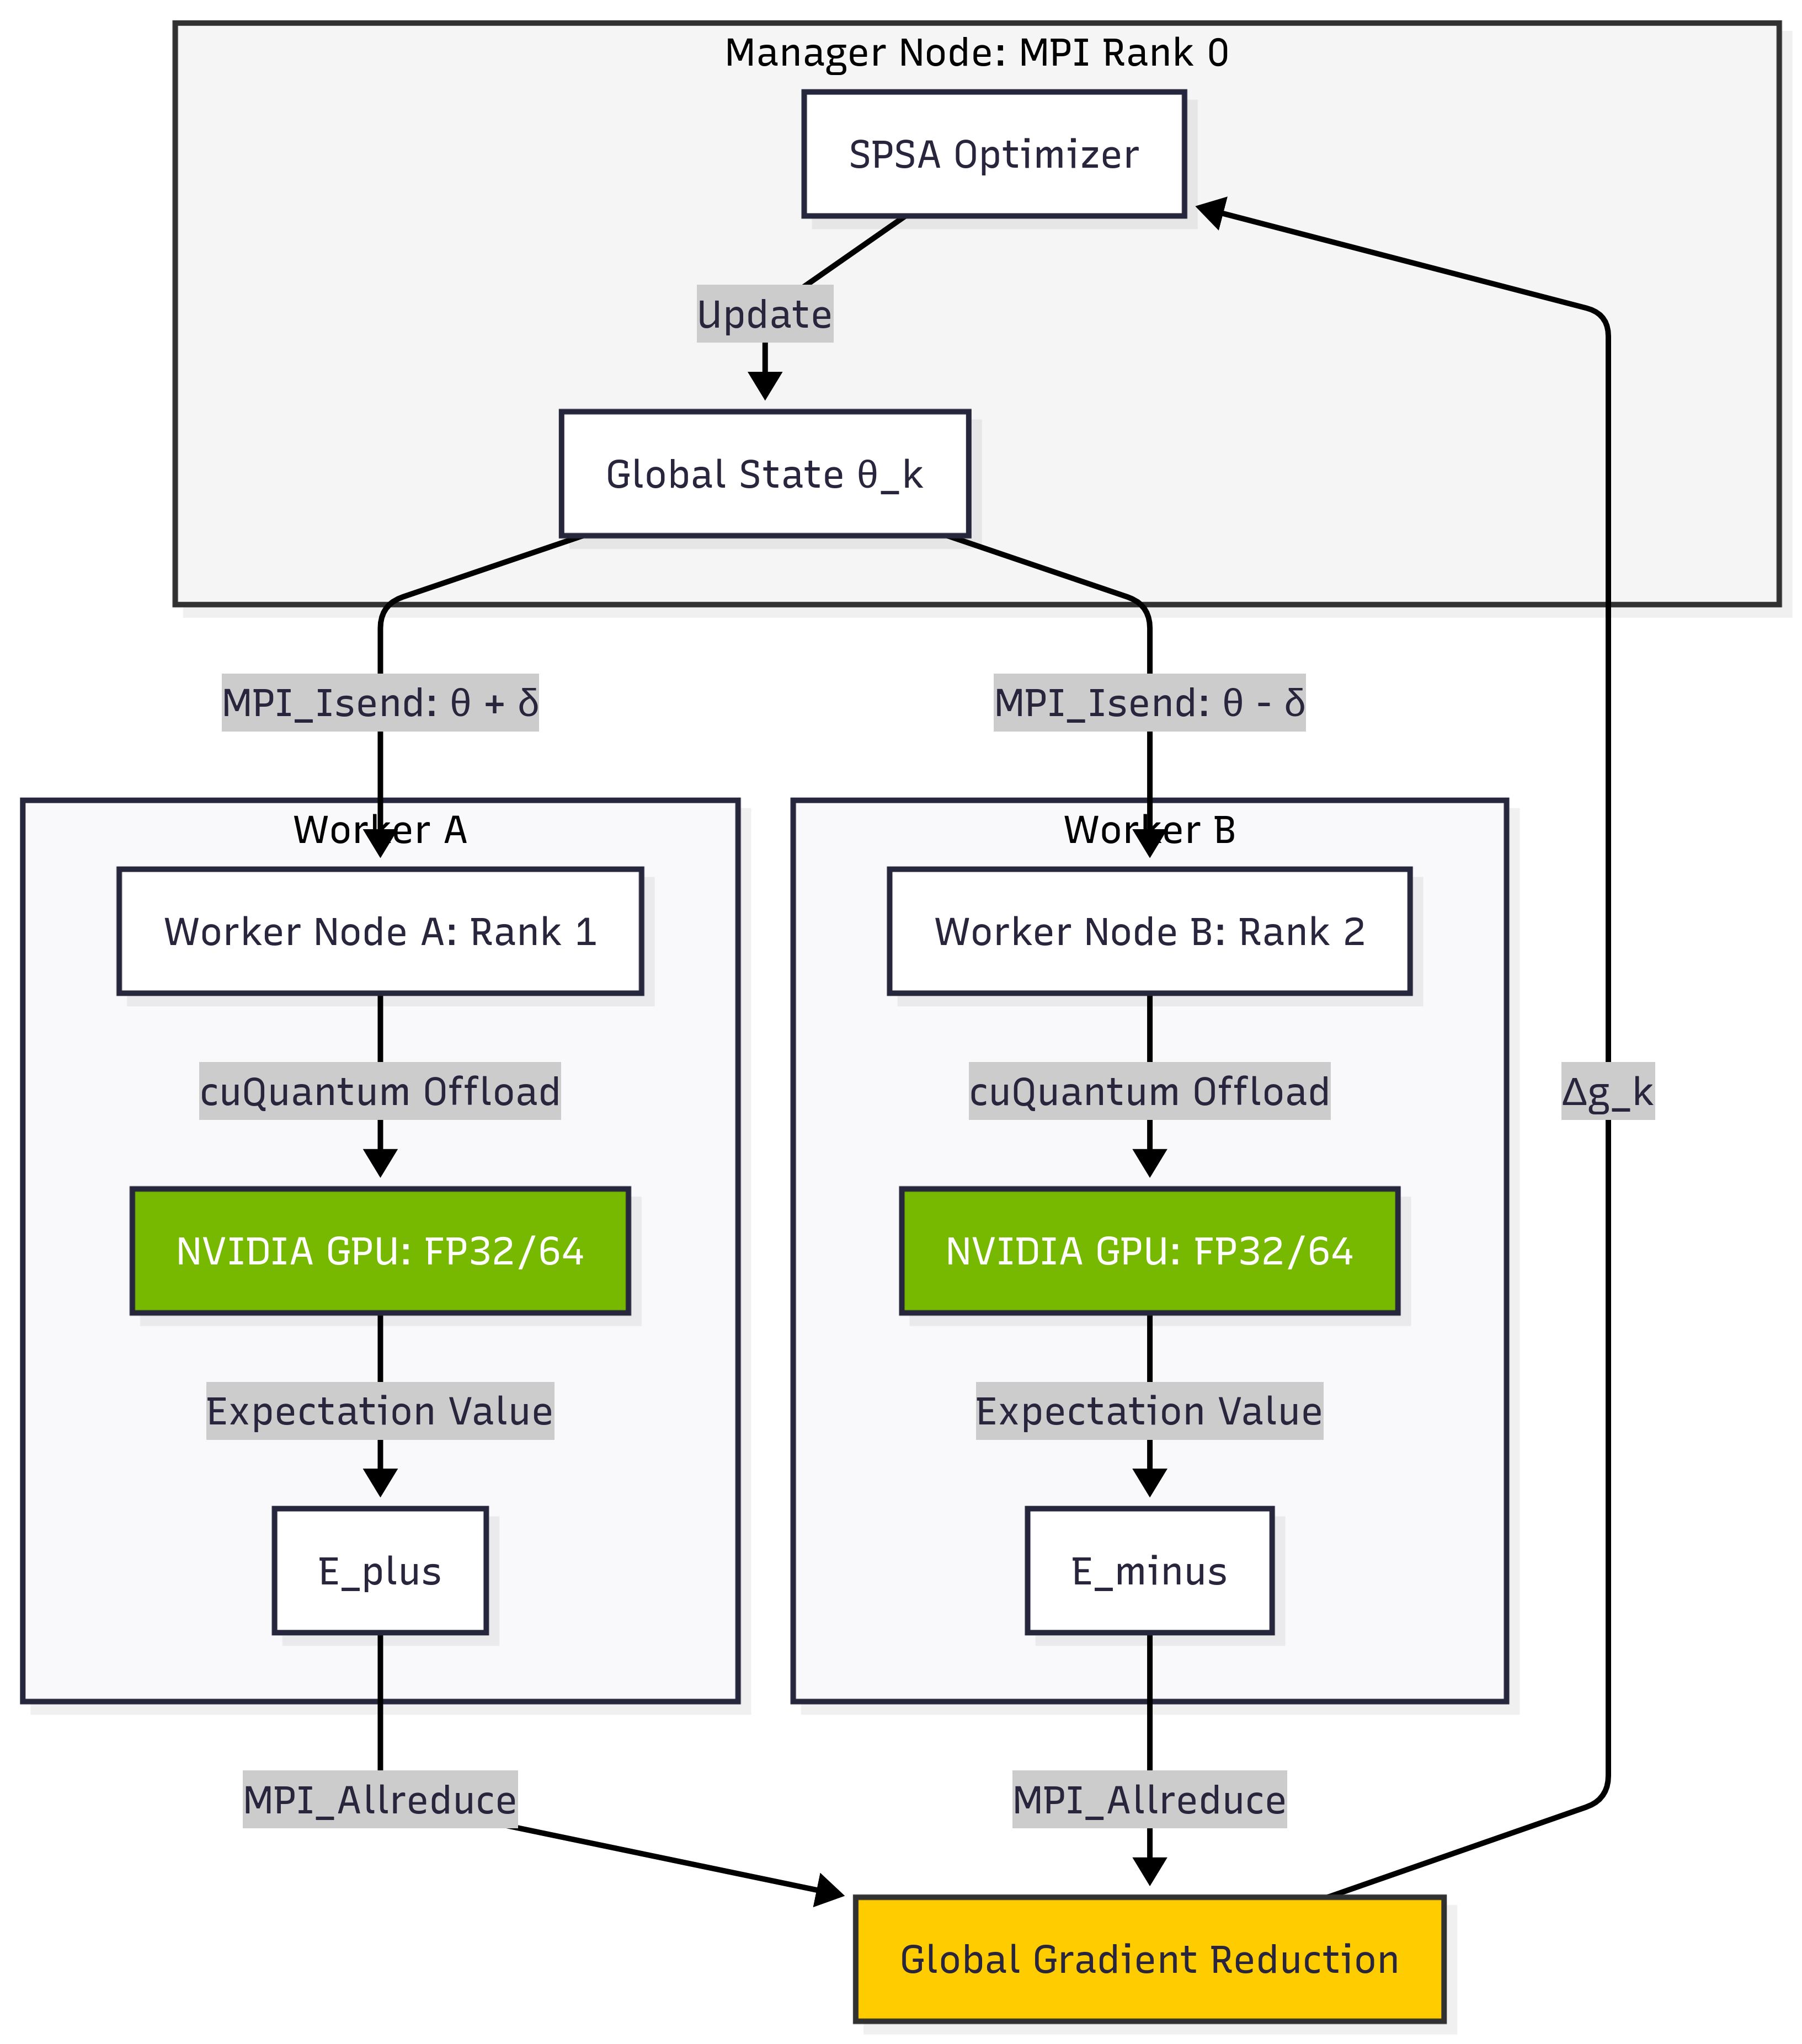
\includegraphics[width=0.8\textwidth]{graphics/spsa_topology.png} 
    \caption{Distributed SPSA Topology}
    \label{fig:spsa_topology}
\end{figure}


\subsubsection{Acceleration Layer: Intra-Node CUDA-Kernel Execution}
This layer follows the findings of Bayraktar et al. \cite{bayraktar2023cuquantum} and is designed in order to offload the computationally heavy $2^n$ state-vector math to each MPI rank's NVIDIA GPU. The stack implements a tiered acceleration strategy with an automatic fallback in place:

\begin{enumerate}
    \item \textbf{GPU statevector (cuStateVec)}: When an NVIDIA GPU is detected, the stack switches to use Qiskit Aer's GPU-accelerated statevector simulator backed by NVIDIA's cuStateVec library from the cuQuantum SDK. This accelerates the $O(2^n)$ statevector construction, which dominates per-iteration cost.
    \item \textbf{CUDA Pauli kernel}: A custom CUDA kernel computes the Pauli term expectation values using a mean-field approximation, with one GPU thread per Pauli term and tree reduction in shared memory. This kernel processes the distributed Pauli terms that are assigned to each MPI rank.
    \item \textbf{CPU fallback}: When no GPU is available, the stack falls back to Qiskit's CPU-based \texttt{Statevector} class for exact state-vector simulation. 
\end{enumerate}

The CUDA kernel adopts a Mixed Precision strategy using FP32/FP64 (32-64 bit floating-point), balancing the stacks need for high computational throughput with  numerical accuracy. FP32 (Single Precision) handles the trigonometric computations of \texttt{cosf} and \texttt{sinf} within each occuring Pauli term evaluation, which provides up to 2x faster throughput on the GPU cores. FP64 (Double Precision) is used for the implemented tree reduction and global accumulation phases in order to prevent precision loss that can occur during the summation of many small contributions. The MPI \texttt{Allreduce} aggregation also operates within FP64, ensuring that the final energy estimate maintains a full double precision accuracy across all ranks.


\subsubsection{Quantum Interface Layer - Asynchronous Dispatcher}
This layer conducts the abstraction of the hardware specific drivers and handles job submission to both local simulators and cloud based QPU backends. Two complementary dispatch paths occur:

\begin{enumerate}
    \item \textbf{C++ dispatcher} (\texttt{dispatcher.cpp}): Manages the MPI synchronization with \texttt{MPI\_Bcast} for parameter distribution and \texttt{MPI\_Allreduce} for the following energy aggregation. Routes computation to either the CUDA Pauli kernel (when GPU is available) or to the CPU mean-field fallback path. For the cloud QPU path, it uses \texttt{std::async} for non-blocking job submission via REST client (\texttt{qpu\_client.cpp}) that then handles IBM Quantum's IAM authentication, JSON payload construction, and polling with exponential backoff.

    \item \textbf{Python EstimatorV2 path} (\texttt{interface.py}): For IBM Quantum experiments, the stack uses Qiskit's EstimatorV2 primitive, which provides the stack with built-in transpilation, observable layout mapping, along with T-REx measurement error mitigation. Both the $E(\theta^+)$ and $E(\theta^-)$ gradient estimations are bundled into one job as two Primitive Unified Blocs (PUBs), therefore reducing the number of QPU round-trips by 50\%. During the QPU wait time, all MPI ranks concurrently compute exact statevector expectation values, providing both a noise-free reference estimate and useful classical work that contributes to the masking metric $M$.
\end{enumerate}

This dual path design allows the stack to determine and then utilize the most appropriate interface for each backend, chosing either the high level Python path for cloud QPU access (with its built-in error mitigation strategy), or the low level C++ dispatcher to better handle high-throughput local computation with GPU acceleration.


\subsection{Algorithmic Workflow: Parallelized VQE}
The Variational Quantum Eigensolver algorithm is reformulated in this stack in order to exploit its distributed nature, following an iterative cycle of: 

    \begin{enumerate}
        \item Global Parameter Broadcast: The optimizer rank broadcasts a vector of parameters ($\theta$) to $P$ parallel nodes.

        \item Parallel Expectation Value Estimation: Each node ($p \in P$) compute the subset of the Pauli string expectation values: $$\langle\psi(\theta)|\hat{O}_i|\psi(\theta)\rangle$$ This is the stacks primary point of parallelization in which $O_i$ terms are distributed across the HPC cluster.

        \item Asynchronous Handshake: When using the cloud QPU backend, circuits queue on the remote processor while the classical MPI ranks will concurrently compute the exact statevector expectation values locally. This overlap provides both noise-free reference estimate and classical work that masks the QPU round-trip latencies.

        \item Reduction and Updating: Expectation values get aggregated using \texttt{MPI\_Allreduce}, then the classical components compute the next $\theta$ for the following iteration.
    \end{enumerate}


\subsection{Performance Evaluation and Experimental Design}
This section describes the full evaluation of this middlware stack, validated through a Strong Scaling analysis, which measures the stack's performance when total problem size is kept fixed while the number of cores is varied \cite{cuboulderScaling}. Strong scaling measures the parallelization efficiency in a fixed environment, therefore Weak Scaling analysis is also implemented to test the middleware's communication overhead to determine if it grows sublinearly as the system scales. 


\subsubsection{Experimental Configuration}  
All simulator experiments of this stack were conducted inside of a Docker container (CUDA toolkit 12.2, Qiskit 2.1+, qiskit-ibm-runtimme 0.45.1, Python 3.11, PySCF 2.4+, OpenMPI from Ubuntu 22.04 system package) on a single host machine Intel Core i7-1065G7 (Ice Lake, with 4 physical cores and 8 logical threads) clocked at 1.30 GHz base, 3.90 GHz turbo with 32 GB RAM, running on Linux Mint. This configuration is done to ensure reproducibility across computing devices. In order to measure strong scaling under the shared memory conditions, the MPI ranks  $P \in \{1,2,4,8\}$ were evaluated on a single host and all results represent a lower bound of the speedup achievable within dedicated multi-node hardware that is connected through Infiniband. 

The SPSA optimizer of the VQE is configured with a fixed pertubation size $c = 0.1$ that can appropriately handle varational angles within $[0,2\pi]$ with a step size of $a=0.628 / \sqrt{p/8}$, which scales inversely with the square root of the number of variational parameters. $A = 0.1 \times \text{max\_iterations}$, the stability constant, delays any aggressively early updates while the decay exponents of $\alpha= 0.602$ and $\gamma = 0.101$ follow the standard schedule of SPSA. The per-iteration update rule is:
\begin{equation}
    a_k = \frac{a}{(k + A)^\alpha}, \quad c_k = \frac{c}{k^\gamma}
\end{equation}
Convergence is determined by a sliding window of 10 iterations and the optimizer terminates when $\max(E) - \min(E) < \tau$ within that window (as $\tau = 1.6$ mHa : the chemical accuracy threshold). An enforced minimum iteration count of $\max(10, \min(2p, 50))$ is applied to prevent false convergences from occuring on the small, early steps. A maximum iteration count scales alongside the number of parameters with $\max(200, 8p)$. For reproducibility, all experiments use a fixed random seed of 42. 

The ansatz configuration that is implemented within the stack is a tiered ansatz system that selects based on a correlation score metric. All four of the benchmark molecules fall within the tier of \texttt{hwe\_adaptive} tier (within correlation scores 0.34--0.50), using the EfficientSU2 circuit with full entanglement and $\min(\text{reps}+1, 3)$ number of repetition layers. The variational parameters use a uniform distribution during initialization ($\mathcal{U}(-0.1, 0.1)$), in order to keep the initial HWE state close to the Hatree-Fock reference $|0\ldots0\rangle$ under the Jordan-Wigner mapping to delay the occurance of particle number violations.  

All quantum backend experiments utilize IBM Quantum’s open access plan, which provides the 156 qubit \texttt{ibm\_marrakesh} processor. The Qiskit IBM Runtime EstimatorV2 primitive is configured with 4096 shots per circuit and with a resilience level 1 (T-REx measurement error mitigation). The GPU-accelerated experiments using NVIDIA GPUs with cuStateVec are architecturally supported within the stack's design and ADD GPU RESULTS WHEN OBTAIED.  

\subsubsection{Application Scenarios}
To demonstrate the effectiveness of this middleware when dealt a scientifically meaningful workload, this project focuses on quantum chemistry and computing the molecular electronic ground-state energies with the VQE. Chemistry was selected as the application for this middleware due three main reasons: firstly, the molecular Hamiltonian maps naturally to a qubit operator through the Jordan-Wigner transformation, which produces a clearly defined set of Pauli terms to then be distributed across MPI ranks (while still not exceeding the coherency limitations of modern day QPUs). Secondly, it was chosen due to the problem size scaling predictably with the number of electrons and basis functions to allow for controlled experiments (ranging from 4-14 qubits). Lastly, it was selected due to the prexisting Full Configuration Interaction (FCI) energies which provide verified ground-truth references for each molecule to be compared to, in order to understand the stacks accuracy. 

From the STO-3G minimal basis set, four molecules of increasing complexity were identified to be benchmark targets for this middleware. Together, these molecules progressively provide a sufficiently complex Hilbert space that can test the efficiency of the MPI/CUDA distribution while still not exceeding the coherency limitations of modern day QPUs. 

\begin{table}[htbp]
\centering
\renewcommand{\arraystretch}{1.4}
\begin{tabular}{|l|c|c|c|c|}
\hline
\textbf{Molecule} & \textbf{Electrons} & \textbf{Qubits} & \textbf{Pauli Terms} & \textbf{FCI Energy ($E_h$)} \\ \hline
H\textsubscript{2} & 2  & 4  & 15   & $-1.1373$ \\ \hline
LiH & 4  & 12 & 631  & $-7.8825$ \\ \hline
BeH\textsubscript{2}  & 6  & 14 & 666  & $-15.5951$ \\ \hline
H\textsubscript{2}O & 8  & 14 & 1086 & $-75.0124$ \\ \hline
\end{tabular}   
\caption{Benchmark molecules with STO-3G basis.  FCI energies computed with the PySCF Full Configuration Interaction solver.}
\label{table:molecules}
\end{table}   

The progression that occurs from the molecule $H_2$ (4 qubits, 15 Pauli terms - fits within the memory of a single MPI rank) to $H_{2}O$ (14 qubits, 1086 Pauli terms) stresses each layer of the middleware. This includes parameter broadcasting, Pauli term partitioning, statevector construction, and MPI reduction. 

   


\subsubsection{Scaling Strategy}
The objective of Strong Scaling is to reduce the execution time within a fixed total problem size by increasing the number of processors, while considering the ideal time spent on $N$ cores and efficiency. The formula for Ideal Time on N number of cores is \cite{cuboulderScaling}: 
\begin{equation}
    \text {Ideal Time } = \frac{(\text{Measured Time at Lowest Core Count})\text{(Lowest Core Count)}}{N}
\end{equation}

Efficiency provides the metric for the appropriate number of cores for a particular calculation size. Achieving  100\% is often not possible within practice, so a there is a tradeoff point established between the efficiency of the usage of computational resources and of the time spent waiting on the calculations to completed must be determined. The formula for Efficiency is \cite{cuboulderScaling}: 
\begin{equation}
    \text {Efficiency } = \frac{\text{Ideal Time}}{\text{Measured Time}}
\end{equation}

In addition to Strong Scaling, Weak Scaling is evaluated, where the molecule (and Hamiltonian's Pauli term count) is increased proportionally alongside the number of MPI nodes ($P$). At each rank count, a molecule is selected that ensure the per-rank workload (terms/rank) remains approximately constant: $H_{2}$ at $P=1$ (15 terms/rank), $LiH$ at $P=2$ (316 terms/rank), $BeH_{2}$ at $P=4$ (167 terms/rank), and $H_{2}O$ at $P=8$ (136 terms/rank). This will test whether the middleware maintains a stable compute-to-communication ratio while the inputted problems scales up towards the `Communication Wall.'


\subsubsection{Stress Test Design}
To ensure a robust asynchronous dispatcher and manager-worker topology, the system will undergo three evaluations using simulations for "Failure Mode": 
\begin{enumerate}
    \item QPU Latency Spiking: A variable delay will be inserted (between 5-30s) into a subset of the worker-rank network calls, done to simulate increased cloud backend latency. This will test the manager ranks ability to rebalance workloads or to be able to maintain a global synchronizations without rank timeouts. 
    \item Mixed Precision Stability: The VQE iterations will raise the number of qubits (approaching 30 qubits) within the simulation in order to monitor the vanishing gradient often caused by FP32 rounding errors. This will determine the threshold at which the system must transition itself to FP64. 
    \item Network Drop-Out Recovery: An intentional SIGKILL will be sent to a worker rank during active job submission to test if the Orchestration Layer can perform a "checkpoint restart", in where the last know global $\theta$ state that is stored in the manager rank is used to resume optimization without a full system crash. Each 5 iterations a checkpoint is saved within checkpoints/ to provide the restart points. 
\end{enumerate}


\subsection{Benchmarking and Measurement Plan}
\subsubsection{Baseline Implementations}
In order to verify the optimized performance of the triple heterogeneous stack, the system is measured against two distinct baselines: 
     \begin{itemize}
         \item Standard Serial Baseline: Execution using Qiskit Statevector VQE on a single core CPU, using identical SPSA hyperparameters, the HWE-adaptive ansatz, and the same convergence criteria as the distributed MPI/GPU stack. This identifies the outcome of the MPI distribution from any algorithmic differences, providing a fair wall-clock comparison that represents the nonoptimized and industry standard starting point.
     \end{itemize}
     \begin{itemize}
         \item Single Node GPU Baseline: Execution using cuStateVec on a single NVIDIA GPU without the MPI distribution, with this baseline done to isolate the speedup contribution from GPU acceleration vs. the multi-node MPI orchestration. ADD HERE ONCE GPU ACCESS IS OBTAINED
     \end{itemize}
 

\subsubsection{Quantitative Metrics}
The primary metric for determining the success of this stack is the observed End-to-End Wall-Clock Time ($T_{total}$). 
   \begin{equation}
    T_{\text{total}} = T_{\text{accel}} + T_{\text{comm}} + T_{\text{quant}}
\end{equation}
Where: 
\begin{itemize}
    \item $T_{accel}$ = time spent on GPU accelerated optimization (classical acceleration).
    \item $T_{comm}$ = overhead from network RTT and MPI synchronization (communication latency).
    \item $T_{quant}$ = QPU execution time (sampling and measurement).
\end{itemize}

\noindent If the quantity of metric $T_{comm}$ is successfully "masked" by the value of the asynchronous $T_{accel}$ execution time, there will be evidence of this stack's progress towards the "quantum advantage" and achievement of the targeted 1.5-3x speedup over standard single node Qiskit workflows.   

\noindent Masking Efficiency ($M$) will be used as a metric for how well the RTT is hidden (masked). 
\begin{equation}
    M= \frac{T_{\text{accel}}}{T_{\text{comm}}}
\end{equation}
If $M \ge 1$, then the classical components completely cover (mask) the communication wait time. 

\noindent To measure the system's ability to handle high volume iterative workloads, Throughput (Circuits per Second) is established as:
\begin{equation}
        \text{Throughput} = \frac{N_{\text{circuits}}}{T_{\text{total}}}
\end{equation}

\begin{table}[htbp]
\centering
\renewcommand{\arraystretch}{1.5} 
\begin{tabular}{|>{\raggedright\arraybackslash}p{3.5cm}|>{\raggedright\arraybackslash}p{1.5cm}|>{\raggedright\arraybackslash}p{4.5cm}|>{\raggedright\arraybackslash}p{3.5cm}|}
\hline
\textbf{Category} & \textbf{Metric} & \textbf{Definition} & \textbf{Success Threshold} \\ \hline
\textbf{System Performance} & $T_{total}$ & End-to-End Wall-Clock Time  & 2--3x speedup vs. Serial Baseline \\ \hline
\textbf{Latency Masking} &   $M$ & Ratio of $T_{accel} / T_{comm}$ & $M \geq 1$ (Full overlap) \\ \hline
\textbf{Throughput} & CLOPS & Circuit Layer Operations Per Second &  $>$ Qiskit serial baseline \\ \hline
\textbf{Hardware Efficiency} & $E$ & Parallel Efficiency ($S/P$) & $\geq 70\%$ at $P=2$ \\ \hline
\textbf{Resource Utilization} & $U_{gpu}$ & Average GPU Occupancy & $\geq 80\%$ during $T_{accel}$ \\ \hline
\textbf{Scientific Fidelity} & $\Delta E$  & Absolute Energy Error (Chemistry) & $\leq 1.6$ mHa (Chemical Accuracy) \\ \hline
\textbf{Resilience} & $R_{time}$ & Recovery Time after Node Failure & $<$ 60 s (Auto checkpoint) \\ \hline
\end{tabular}
\caption{Quantitative Success Metrics for Middleware Evaluation.}
\label{table:success_metrics}
\end{table}


\subsubsection{Parallel Efficiency and Scalability}
This project measures Parallel Efficiency ($E$), calculated as:
\begin{equation}
    E = \frac{S}{P} = \frac{T_{s}}{P \times T_{p}}
\end{equation}
where $P$ represents the number of active MPI nodes, $T_{s}$ is the serial (single core) wall-clock time, $T_{p}$ is the measured parallel wall-clock time, and $S = T_{s}/T_{p}$ is the measured speedup. This metric is used to demonstrate if the "Communication Wall" is being successfully handled as the cluster scales.  

\subsubsection{Correctness and Convergence}
For the purpose of ensuring the optimizations (such as Mixed Precision (FP32/FP64) and SPSA) do not compromise the science of this stack, the tested molecules ground state energy results will be compared against the preestablished Full Configuration Interaction (FCI) results for ground state energies. This software stack is considered successful within the application of quantum chemistry if it maintains Chemical Accuracy ($\approx 1.6$ mHa) throughout the parallelized iterations. 

For broader applications of this software's accuracy, Relative Error  ($\epsilon$) is used: 
\begin{equation}
    \epsilon = \frac{|E_{exact} - E_{stack}|}{|E_{exact}|} 
\end{equation}
This provides an application agnostic accuracy measure that will extends beyond quantum chemistry to any domain (future applications can include Optimization Problems, Fianancial Portfolios, etc.) where the stack can compute variational ground state energies. 



